\subsection{GRPO y la optimización relativa por grupos}
\label{sec:grpo}
Group Relative Policy Optimization (GRPO) genera varias respuestas para una misma consulta y utiliza sus recompensas para estimar una ventaja relativa, evitando entrenar un crítico separado. Si el grupo contiene $G$ respuestas con recompensas $r_1,\ldots,r_G$, una expresión simplificada de esa ventaja es
\begin{equation}
A_i=\frac{r_i-\overline{r}}{\sigma_r+\varepsilon_n},
\qquad \overline{r}=\frac{1}{G}\sum_{i=1}^{G}r_i,
\qquad \sigma_r=\sqrt{\frac{1}{G}\sum_{i=1}^{G}(r_i-\overline{r})^2},
\label{eq:ventaja-grpo}
\end{equation}
donde $\overline{r}$ representa el promedio del grupo, $\sigma_r$ su dispersión y $\varepsilon_n$ un término pequeño de estabilidad numérica. La normalización por la media y la desviación estándar corresponde al mecanismo de la formulación original, mientras que el término añadido y la convención para calcular la desviación pueden variar entre implementaciones~\cite{shao2024deepseekmath}.

Una ventaja positiva favorece un aumento de la probabilidad de la respuesta respecto de la política de recolección, mientras que una negativa produce el incentivo contrario, sujeto al objetivo con clipping y a la regularización utilizada. Por lo tanto, importa la diferencia entre las recompensas y no solamente su promedio, ya que un grupo con recompensas idénticas tiene ventajas relativas nulas bajo la ecuación \ref{eq:ventaja-grpo}, aunque puedan existir gradientes de otros términos del objetivo. La figura \ref{fig:grpo-ejemplo} ilustra este cálculo con cuatro respuestas y valores elegidos únicamente para explicar el procedimiento.

\begin{figure}[htbp]
\centering
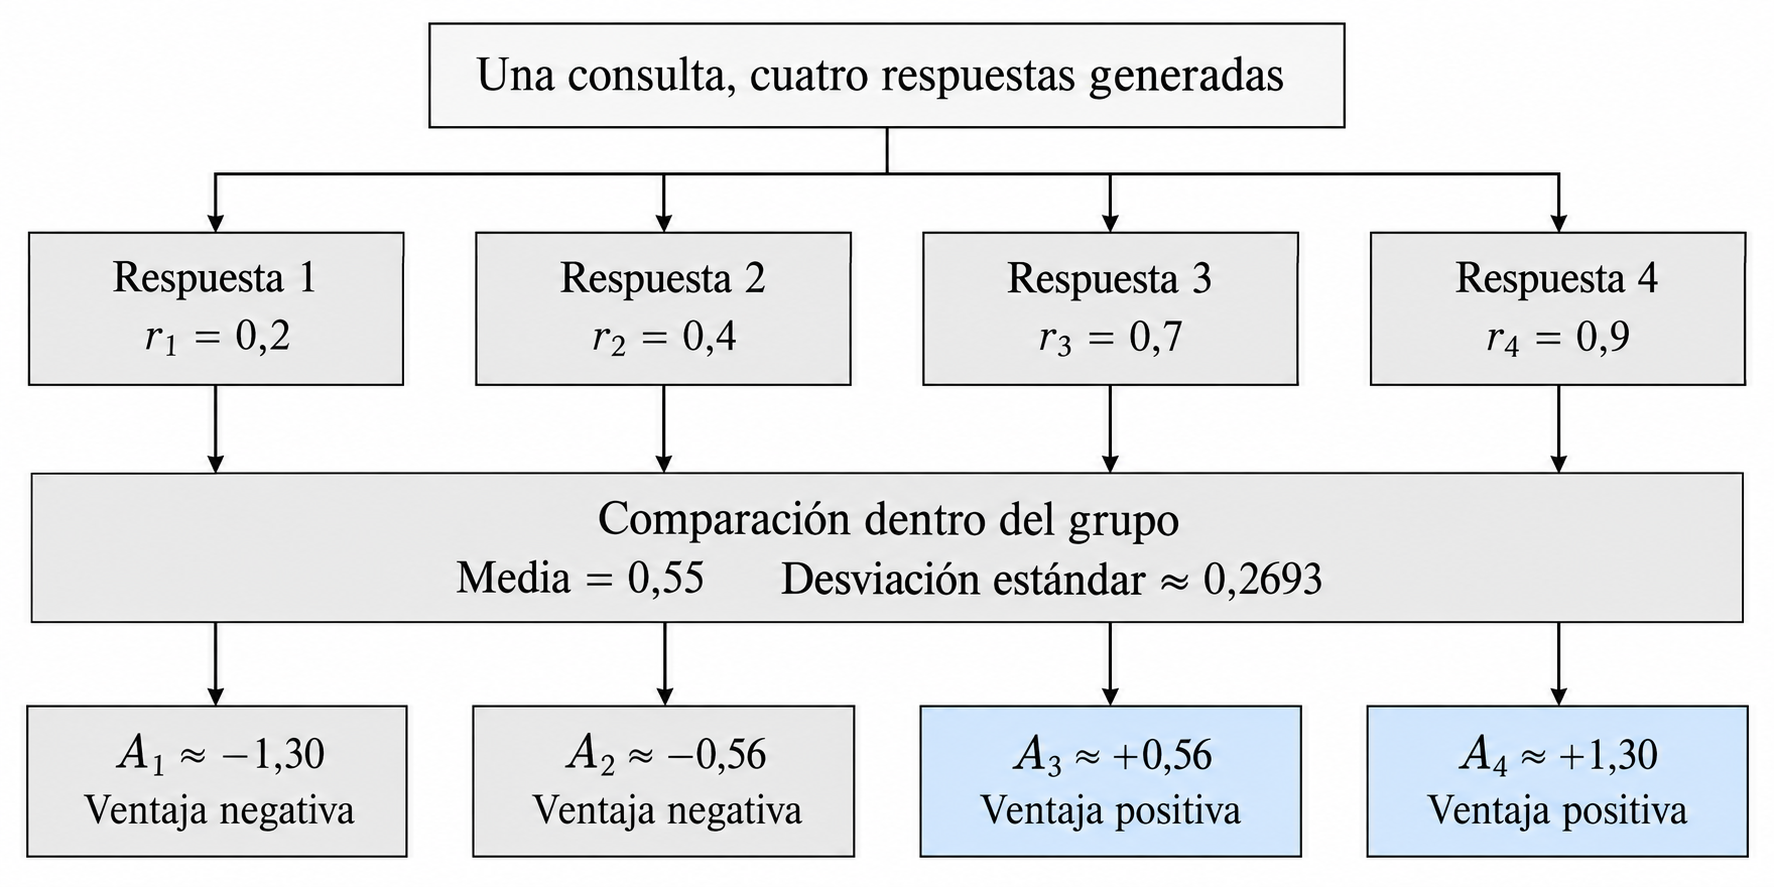
\includegraphics[width=0.95\textwidth]{Figuras/02-marco-teorico/04-ppo-grpo/rl-grpo-grupo.png}
\caption{Ejemplo ilustrativo de comparación de recompensas y ventajas en GRPO.}
\label{fig:grpo-ejemplo}
\end{figure}

Para relacionar esa comparación con la actualización de parámetros, puede escribirse el objetivo de GRPO con recompensa final como
\begin{equation}
\begin{aligned}
J_{\mathrm{GRPO}}(\theta)
&=\mathbb{E}_{x,\{y_i\}\sim\pi_{\mathrm{old}}}\left[
\frac{1}{G}\sum_{i=1}^{G}\frac{1}{T_i}\sum_{t=1}^{T_i}
\left(C_{i,t}(\theta)-\beta D_{i,t}(\theta)\right)\right],\\
C_{i,t}(\theta)
&=\min\left(\rho_{i,t}(\theta)A_i,
\operatorname{clip}(\rho_{i,t}(\theta),1-\epsilon_c,1+\epsilon_c)A_i\right),\\
\rho_{i,t}(\theta)
&=\frac{\pi_\theta(y_{i,t}\mid x,y_{i,<t})}
{\pi_{\mathrm{old}}(y_{i,t}\mid x,y_{i,<t})}.
\end{aligned}
\label{eq:objetivo-grpo}
\end{equation}
En esta expresión, las consultas se extraen de $\mathcal{D}$ y las respuestas se generan con la política de recolección, mientras que $T_i$ es la longitud de la respuesta $i$ y $D_{i,t}$ representa la divergencia respecto de la política de referencia en el contexto del token $t$. El término $C_{i,t}$ combina la razón de probabilidades con la ventaja y el recorte de PPO, mientras que $\beta D_{i,t}$ penaliza la desviación respecto de la referencia~\cite{shao2024deepseekmath}. Por lo tanto, maximizar este objetivo favorece los tokens de respuestas con mejor recompensa relativa, sujeto a esos mecanismos de control, y la pérdida utilizada para minimizar mediante descenso de gradiente puede definirse como $\mathcal{L}_{\mathrm{GRPO}}=-J_{\mathrm{GRPO}}$. La división por $T_i$ da el mismo peso total a cada respuesta antes de promediar el grupo, una elección que puede cambiar en otras variantes.

Cuando se utiliza una recompensa final, la ventaja de la respuesta puede aplicarse a sus tokens durante la actualización, aunque la formulación también contempla señales de proceso y variantes posteriores modifican la normalización y la ponderación por longitud~\cite{shao2024deepseekmath,deepseek2025r1}. En consecuencia, documentar que se utilizó GRPO no basta para reproducir una corrida, sino que deben precisarse su variante, la recompensa y las decisiones de implementación. Además, $G$ indica cuántas respuestas se generan por consulta y debe distinguirse del tamaño del microbatch y de la acumulación de gradientes, definidos en la sección \ref{sec:sft-actualizacion}.

